%\documentclass{article}
\documentclass[]{article}
\usepackage{bm}
\usepackage{amsmath}
\usepackage{amsfonts}
\usepackage{natbib}
\usepackage{graphicx}
\usepackage{placeins}
\bibliographystyle{unsrtnat}

\begin{document}



\section{Short update}
\begin{itemize}
	\item Last call: impact of a payroll tax cut / extension of unemployment benefits on consumption; there were no aggregate demand effects
	\item Edmund created code to capture AD effects: Current consumption affects TFP: $TFP_t = \left(\frac{C_t}{C_{ss}}\right)^\alpha$ where $\alpha = 0.4$.
	\item What is working so far: AD effects for payroll tax cut experiment, for recession and for payroll tax cut during recession
	\item What is not working yet: AD effects for unemployment benefits extension
\end{itemize}

\section{Stimulus Experiments}

Parametrization
\begin{itemize}
	\item Update probabiltity = 1 (have not tried sticky information yet)
	\item 7 discount factor groups: Beta = 0.986 (center), Nabla = 0.0183 (spread) as estimated on Norwegian Data
	\item Splurge = 0.32 as estimated on Norwegian Data
	\item Simulation of these results takes about 4 h (50k Agents, T-sim = 400)
\end{itemize}	

\subsection{Recession}

\begin{itemize}
	\item We consider a recession with an expected length of 6 quarters, see Figure \ref{fig:recession}
	\item In a recession the unemployment rate increases to 10 \% and lasts on average 4 quarters (as opposed to 5\% / 1.5 q in normal times)
	\item The recession depresses aggregate income due to loss of labor income, only partly compensated by unemployment benefits (lasting 2 q, replacing 30 \% of income)
	\item Consumption falls as income is lower.
	\item The recession is deeper when productivity depends on aggregate demand.
\end{itemize}


\begin{figure} 
	\begin{centering}
		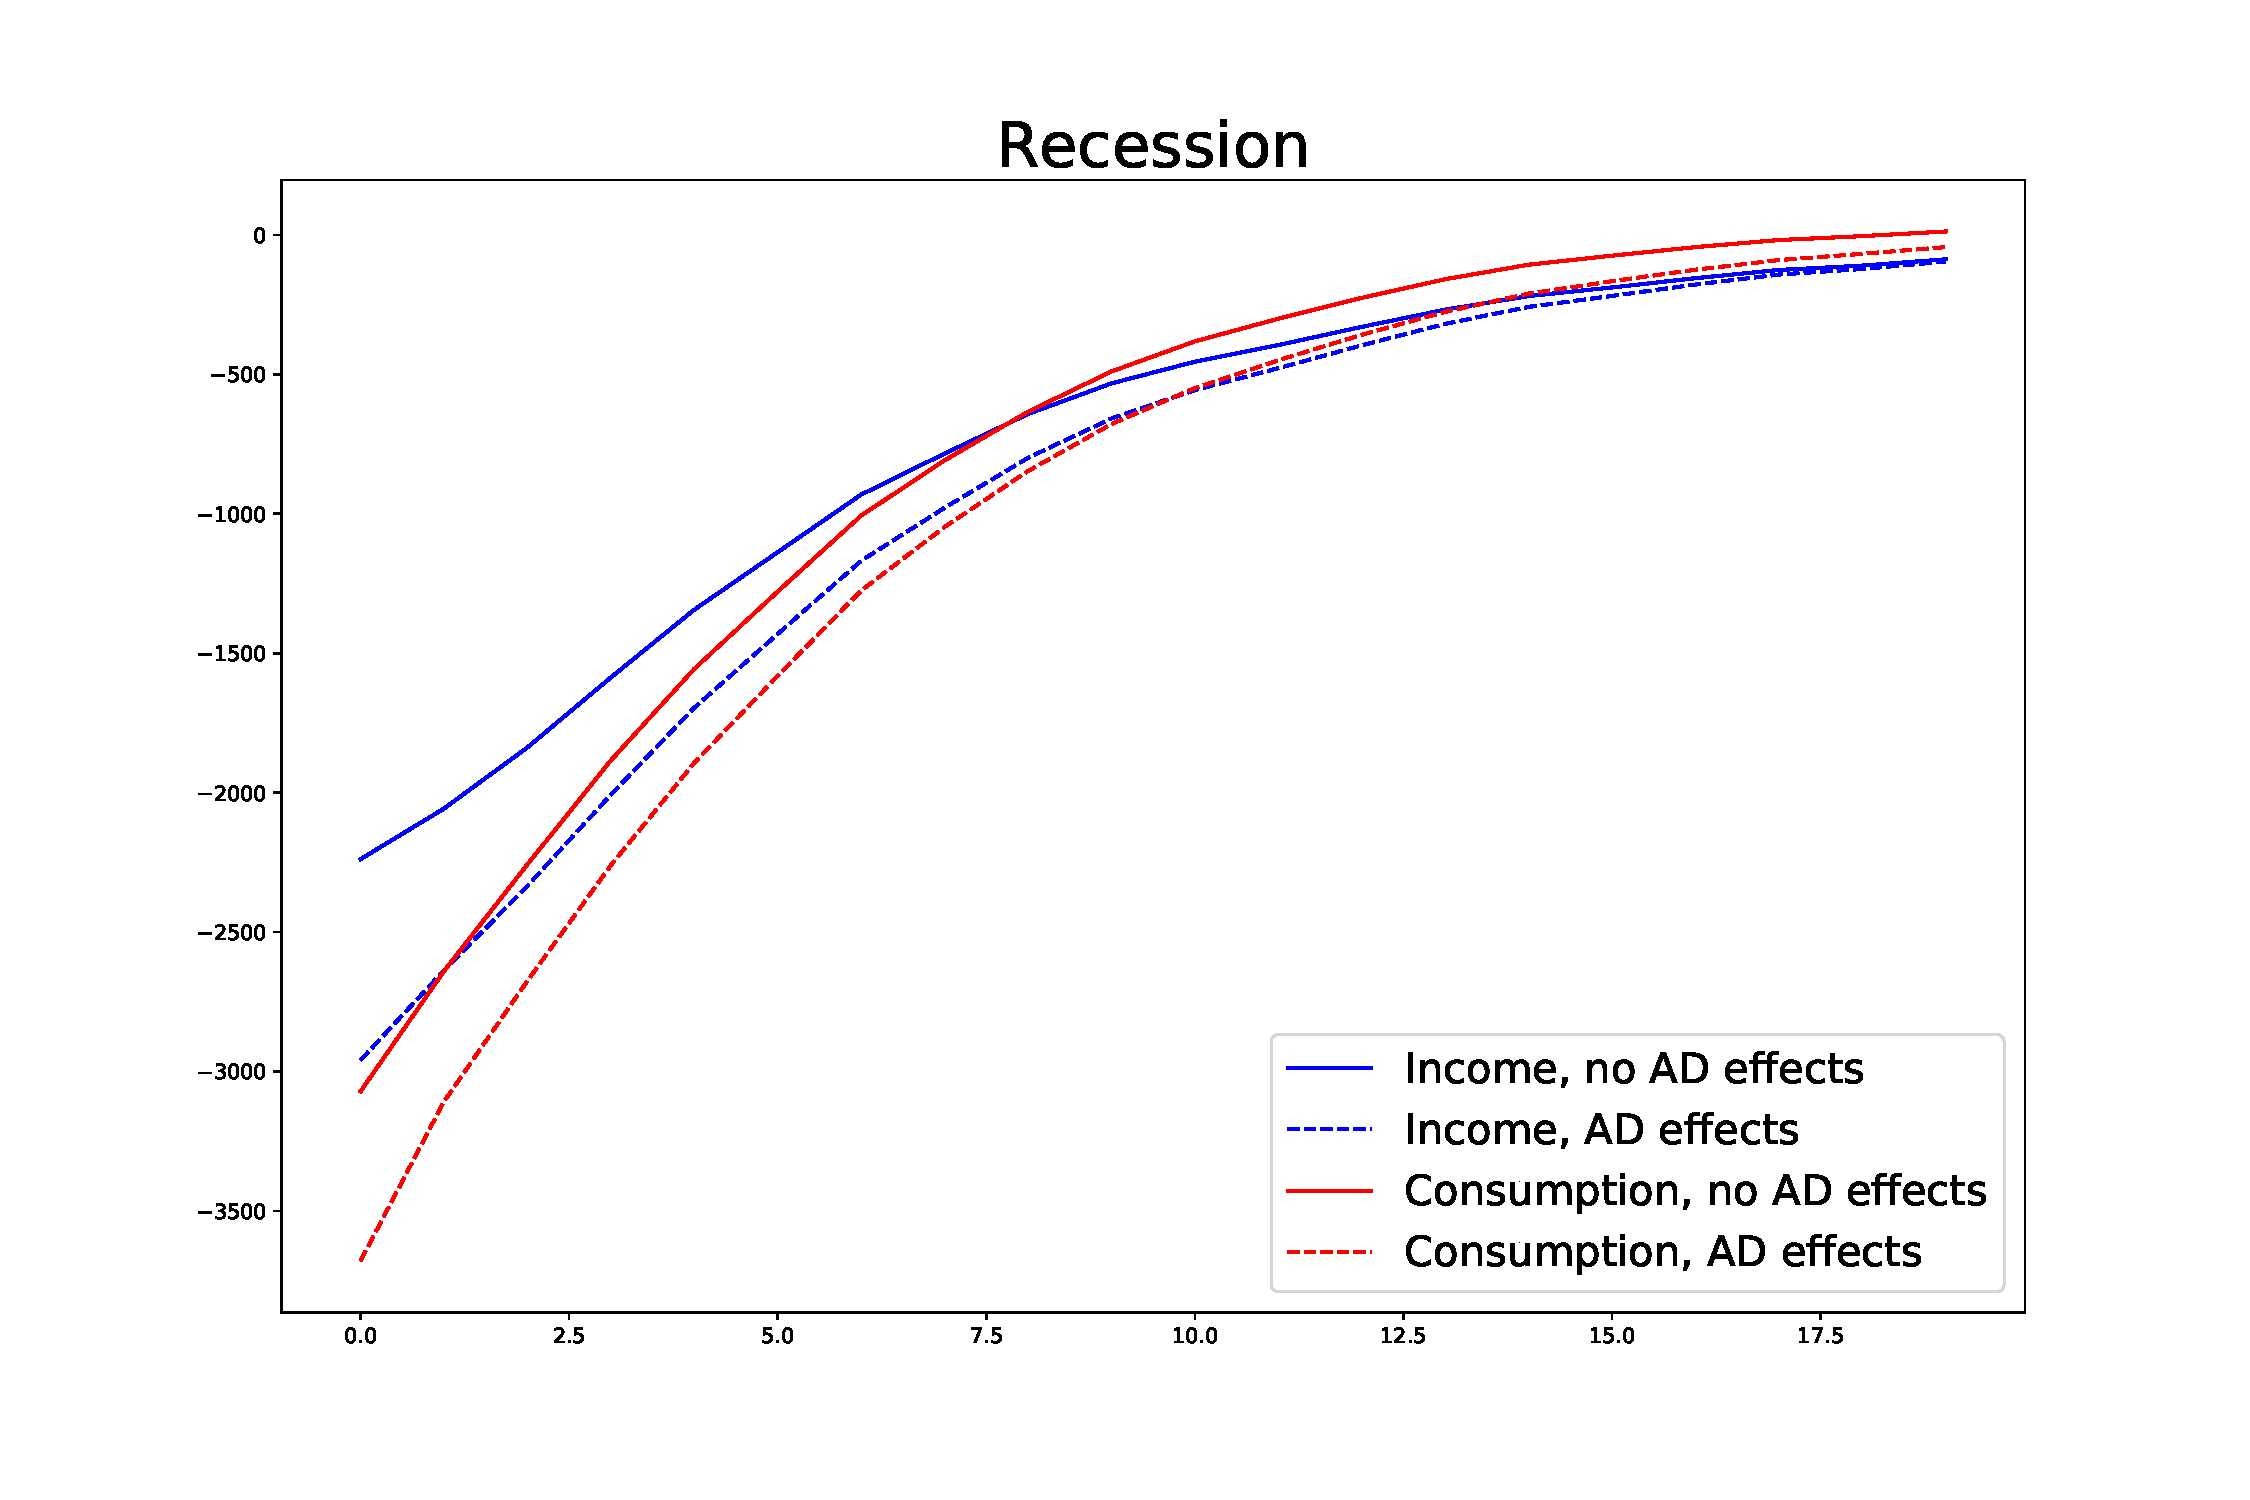
\includegraphics[width=\linewidth]{../recession.pdf}
		\caption{Recession}
		\label{fig:recession}
	\end{centering}
\end{figure}

\FloatBarrier
\subsection{Tax cut}

\begin{itemize}
	\item We consider a payroll tax cut by 2 pp for 8q (deterministic length)
	\item See Figure \ref{fig:taxcut}
	\subitem The tax increases income and consequently pushes up consumption
	\subitem The drop in consumption in 9q is due to the fact that the splurge is applied to income in excess of the baseline income, which drops to zero after the tax cut is reversed. Consumption spending remains elevated for some time after the tax cut due to built up savings. 
	\subitem With aggregate demand effects, the effect on consumption is larger as the increased consumption reinforces consumption through higher income due to higher TFP	
\end{itemize}

\begin{figure} 
	\begin{centering}
		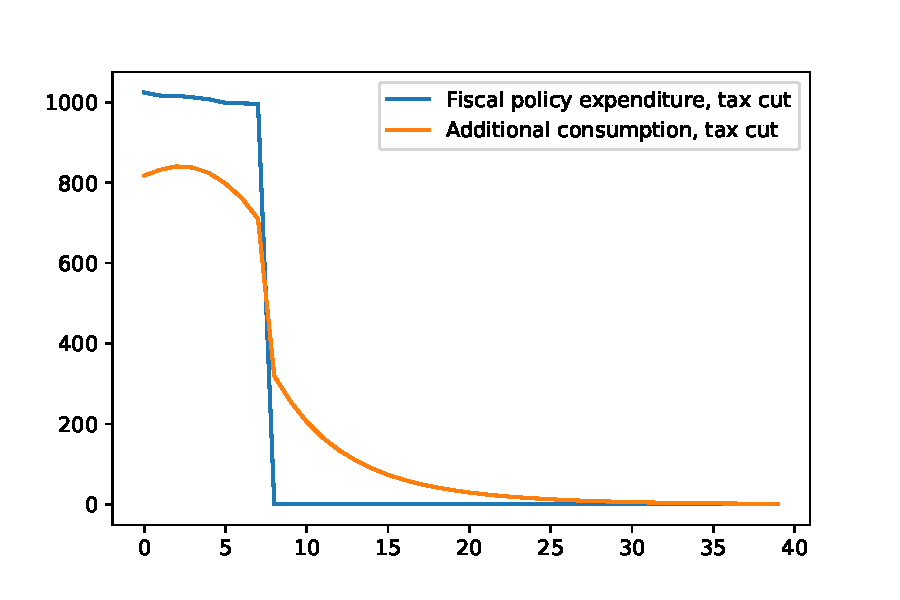
\includegraphics[width=\linewidth]{../tax_cut.pdf}
		\caption{Tax cut}
		\label{fig:taxcut}
	\end{centering}
\end{figure}

\FloatBarrier
\subsection{Tax cut during recession}

\begin{itemize}
	\item We consider a payroll tax cut by 2 pp for 8q (deterministic length) during a recession with an expected length of 6q 
	\item Additional income / consumption relative to the baseline (see figure \ref{fig:taxcutrecession}) and to recession scenario (see figure \ref{fig:taxcutrecession2})
	\item When AD effects are switched off we obtain a similar result as in the baseline. However, note, that as the recession disappears, the additional income by the tax cut increases as more people are employed
	\item This upward trend in the effect of the tax cut is much more pronounced when considering AD effects. This is because very low consumption at the beginnning of the recession sets a much steeper recovery path.
	\item Not clear why consumption first drops (numerical error?)
\end{itemize}

\begin{figure} 
	\begin{centering}
		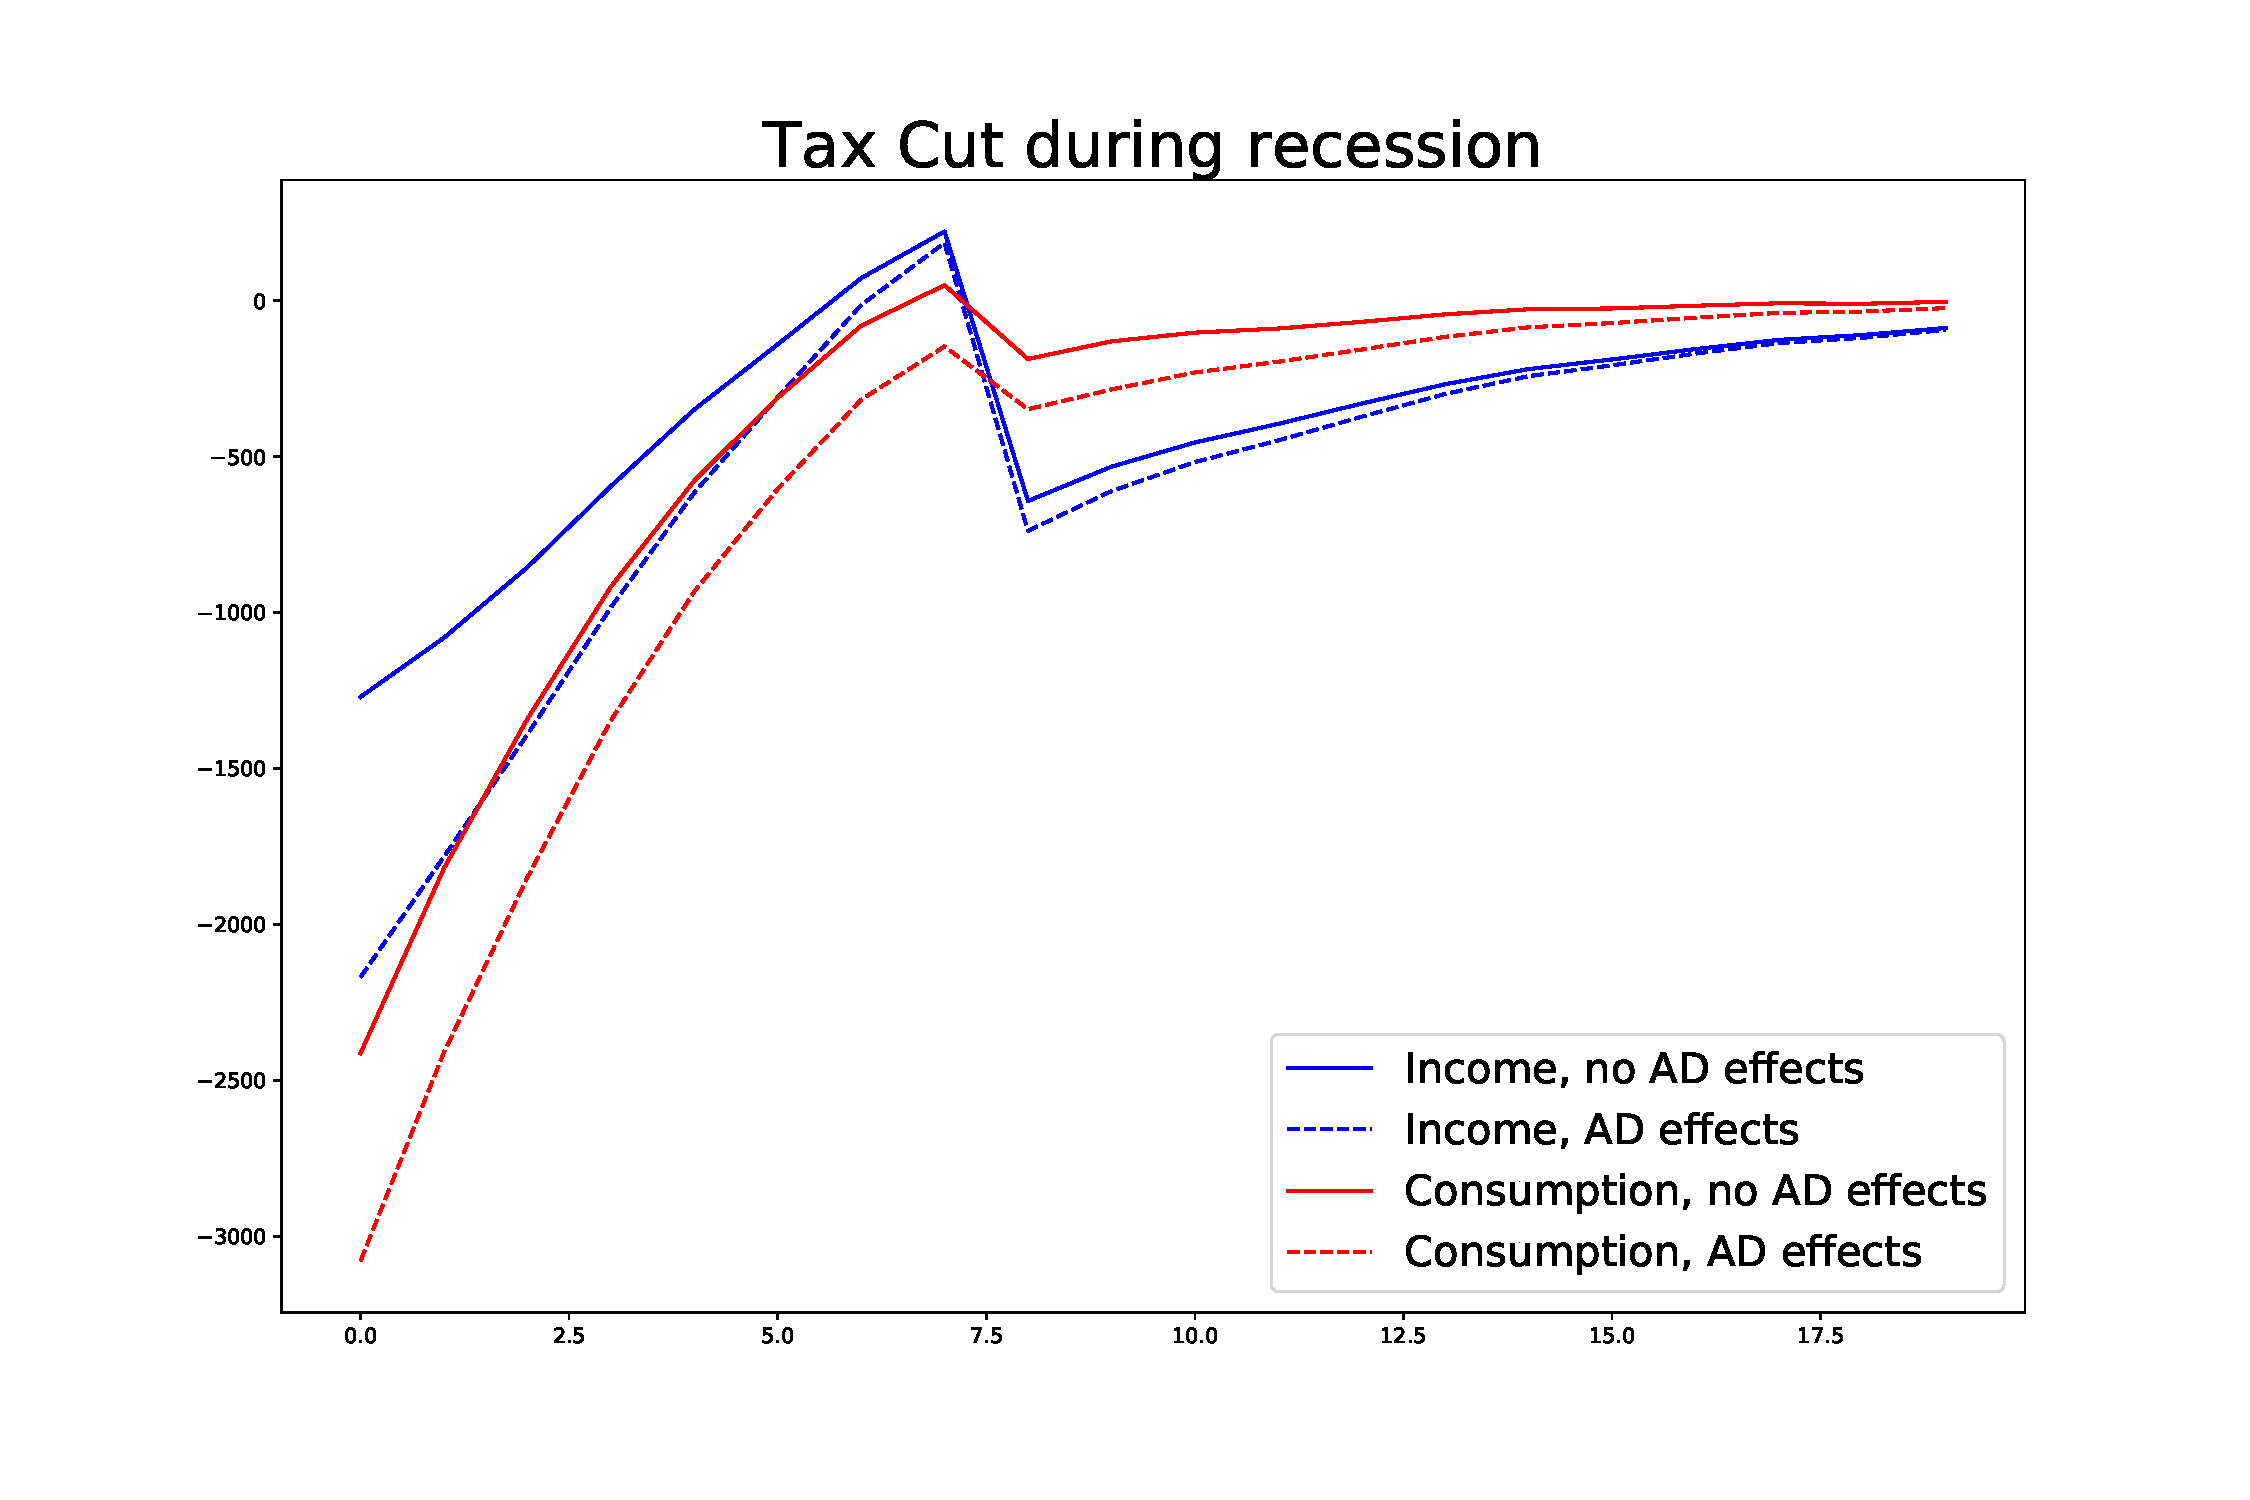
\includegraphics[width=\linewidth]{../taxcut_recession.pdf}
		\caption{Tax cut during a recession}
		\label{fig:taxcutrecession}
	\end{centering}
\end{figure}
\begin{figure} 
	\begin{centering}
		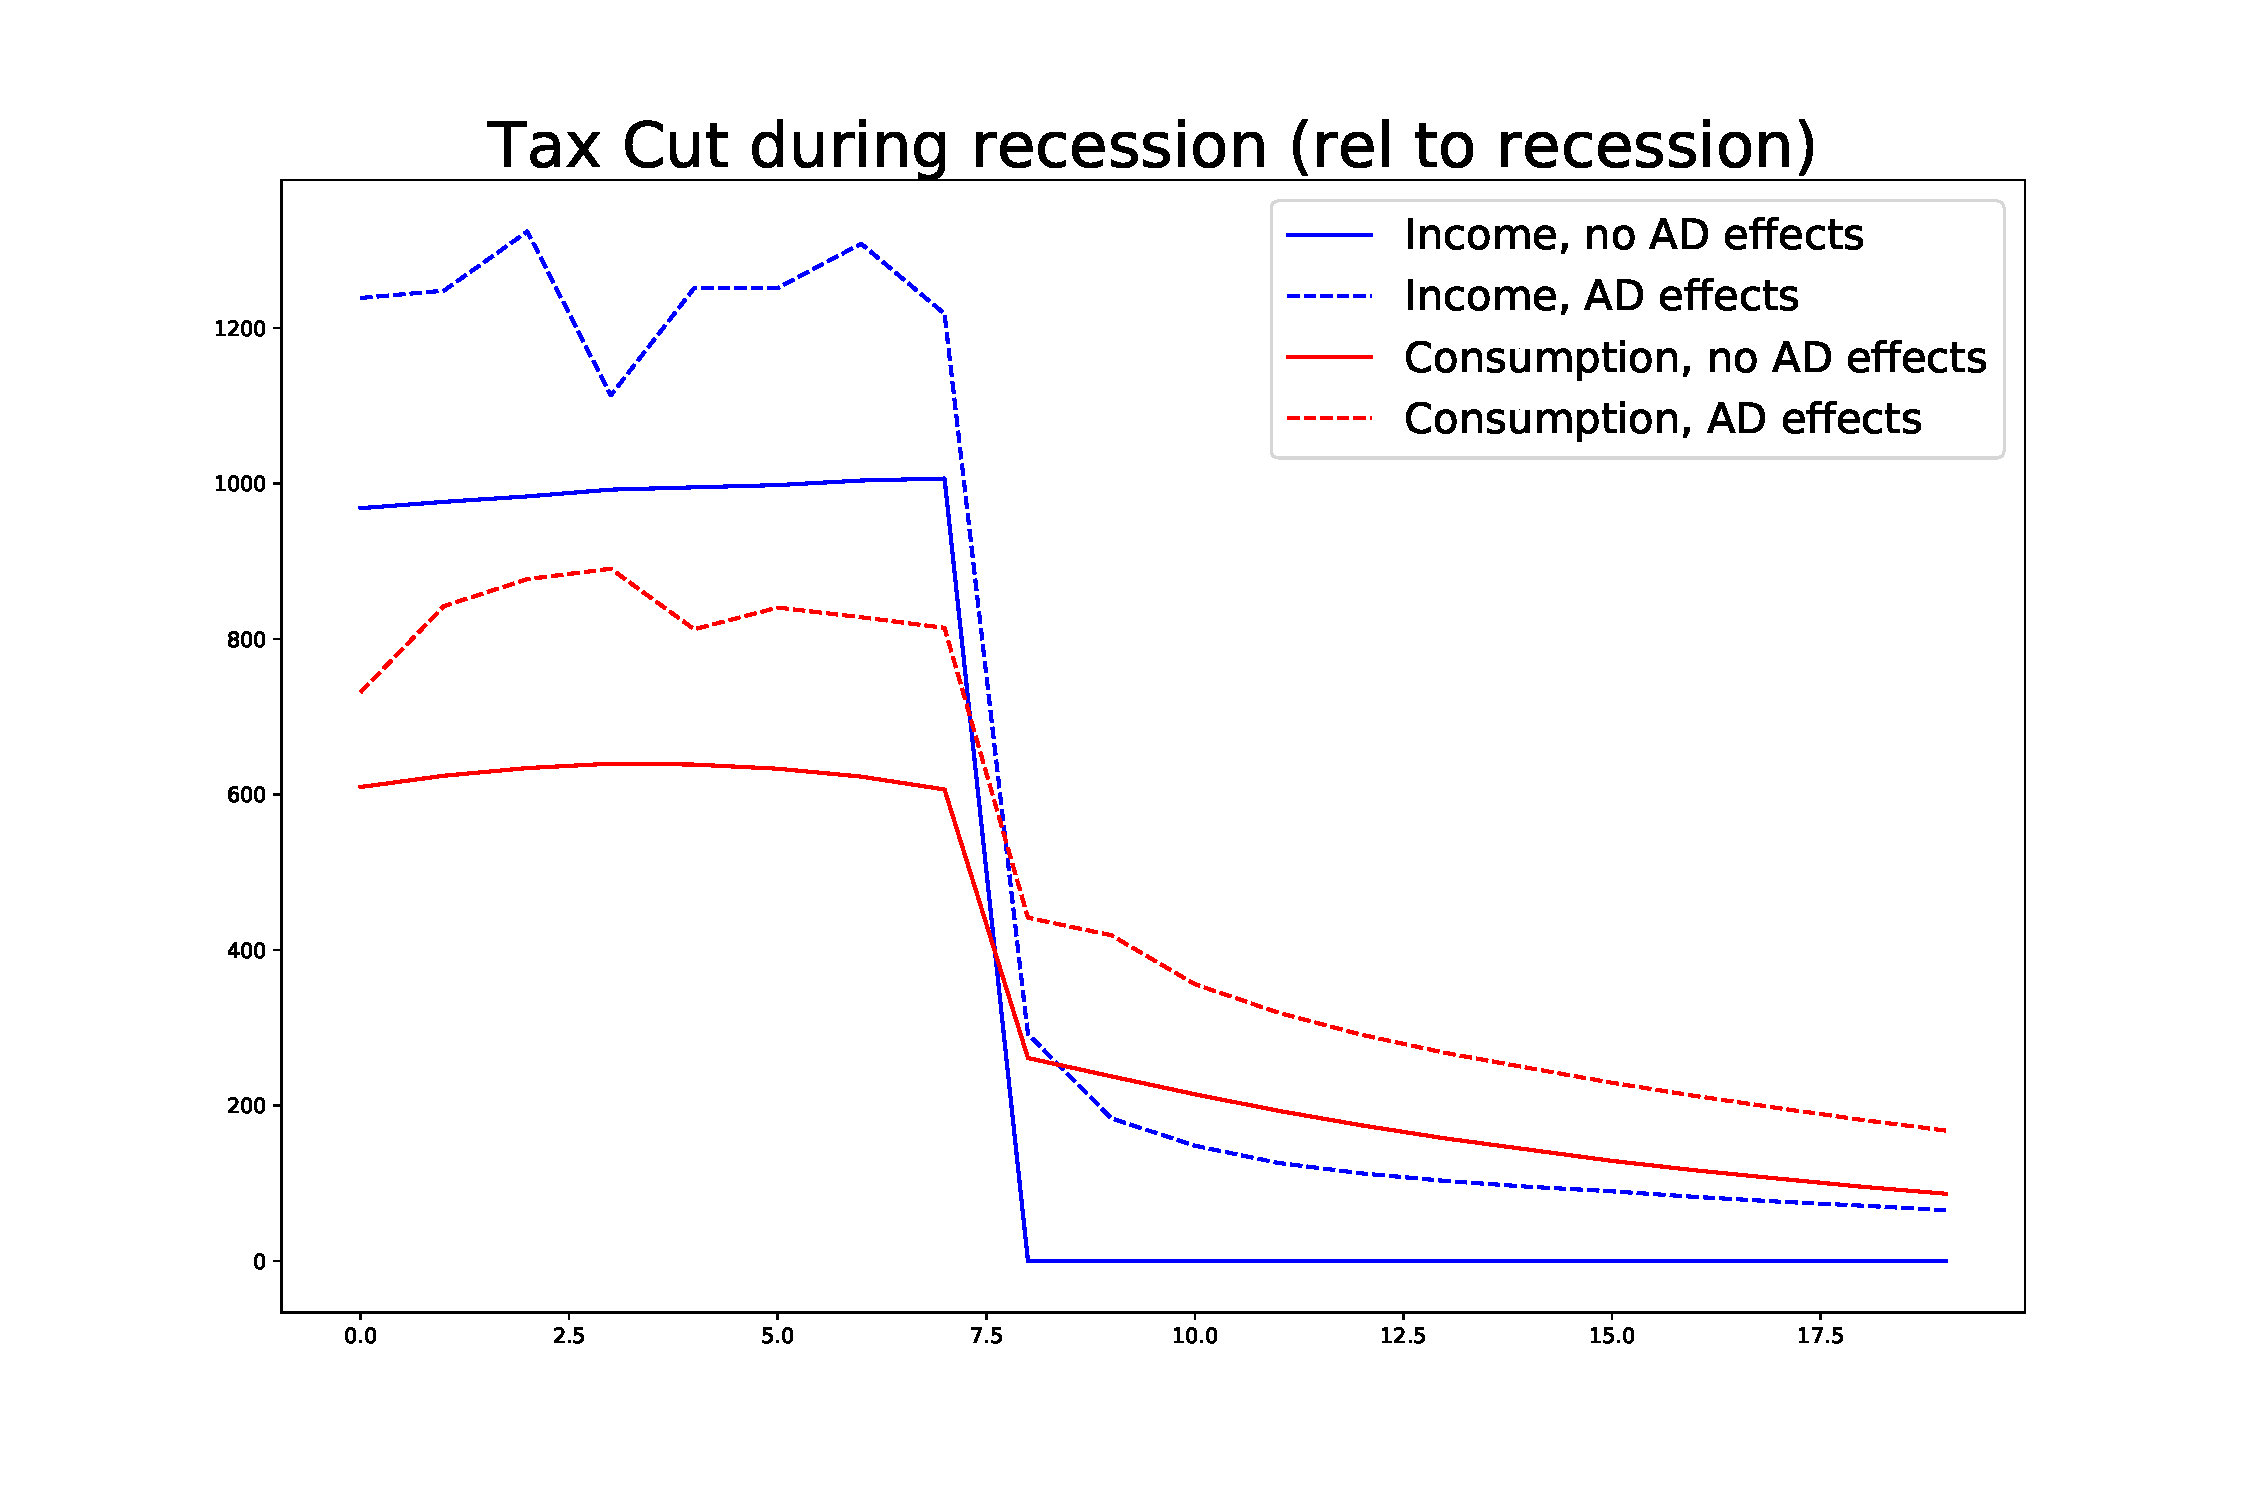
\includegraphics[width=\linewidth]{../taxcut_recession2.pdf}
		\caption{Tax cut during a recession}
		\label{fig:taxcutrecession2}
	\end{centering}
\end{figure}

\FloatBarrier
\subsection{[Preliminary] Comparing magnitude of stimulus relative to policy expenditure}

\begin{itemize}
	\item Figure \ref{fig:stimulus} shows the additional consumption caused by the policy relative to the total net present value of the policy intervention
	\item However, we use the net present value from the no AD scenario
	\item This is problematic, need to calculate the amount of additional expenditure due to the fiscal policy intervention -> 2pp x recession-Ad-income
\end{itemize}

\begin{figure} 
	\begin{centering}
		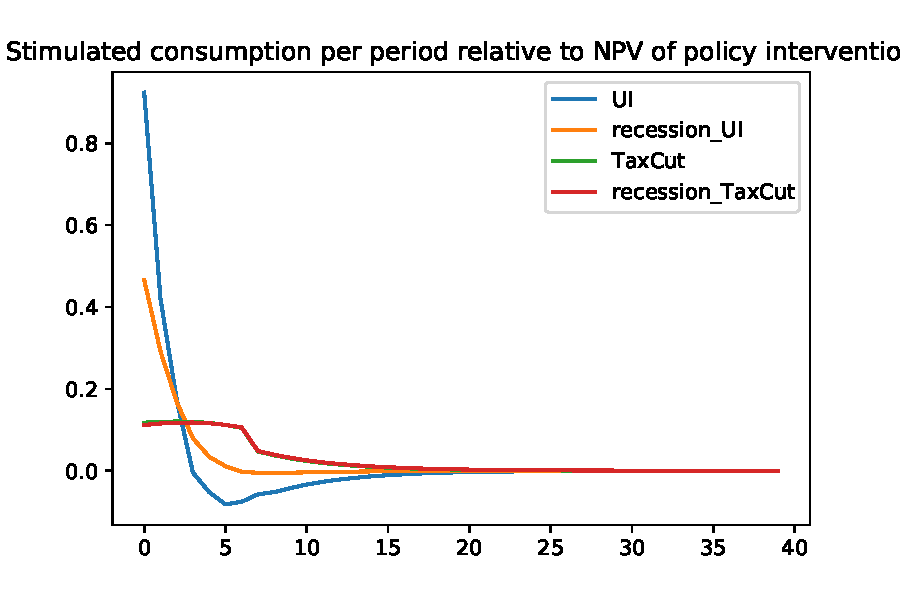
\includegraphics[width=\linewidth]{../stimulated-consumption.pdf}
		\caption{Stimulus}
		\label{fig:stimulus}
	\end{centering}
\end{figure}





\end{document}
